\documentclass[a4paper,oneside,article]{memoir}

\usepackage{microtype}

\usepackage[UTF8]{inputenc}
\usepackage[Danish]{babel}
\usepackage[T1]{fontenc}

\setsecnumdepth{subsection}
\setcounter{tocdepth}{5}
\setcounter{secnumdepth}{4}

%\usepackage{biblatex}
\usepackage{natbib}
\usepackage[hidelinks=true]{hyperref}
\usepackage{lmodern}
\usepackage{parskip}

\usepackage[table,xcdraw]{xcolor}

% For rotating text in tables
\usepackage{array,graphicx}
\usepackage{booktabs}
\usepackage{pifont}

\newcommand*\rot{\rotatebox{90}}
\newcommand*\OK{\ding{51}}

%Billeder skal
\usepackage{graphicx}
\graphicspath{ {Afsnit/} }
\usepackage{float}
\usepackage{wrapfig}
\usepackage{chngpage}

% Listings og color bruges til at vise vores VHDL kode med.
\usepackage{listings}
\usepackage{color}

\usepackage{longtable}
\usepackage{tabularx}

\definecolor{dkgreen}{rgb}{0,0.6,0}
\definecolor{gray}{rgb}{0.5,0.5,0.5}
\definecolor{mauve}{rgb}{0.58,0,0.82}

\lstset{frame=tb,
  language=C++,
  aboveskip=3mm,
  belowskip=3mm,
  showstringspaces=false,
  columns=flexible,
  basicstyle={\small\ttfamily},
  numbers=none,
  numberstyle=\tiny\color{gray},
  keywordstyle=\color{blue},
  commentstyle=\color{dkgreen},
  stringstyle=\color{mauve},
  breaklines=true,
  breakatwhitespace=true,
  tabsize=3
}

%This part is just for fun! Please delete before turn-in
%=======================================================
\usepackage{transparent}
\usepackage{eso-pic}
\newcommand\BackgroundPic{%
	\put(0,0){%
		\parbox[b][\paperheight]{\paperwidth}{%
			\vfill
			\centering
			{\transparent{0.4} \includegraphics[width=\paperwidth,height=\paperheight]{background}}
			\vfill
		}}}
%=======================================================

\title{3. Semesterprojekt - Goofy Candy Gun\\ Gruppe 3}

\author{
  Rieder, Kasper\\
  \texttt{201310514}
  \and
  Jensen, Daniel V.\\
  \texttt{201500152}
  \and
  Nielsen, Mikkel\\
  \texttt{201402530}
  \and
  Kjeldgaard, Pernille L.\\
  \texttt{PK94398}
  \and
  Konstmann, Mia\\
  \texttt{201500157}
  \and
  Kloock, Michael\\
  \texttt{201370537}
  \and
  Rasmussen, Tenna\\
  \texttt{201406382}
  \and
  Vejleder:\\ Gunvor Elisabeth Kirkelund\\
}

\pagestyle{headings}

\begin{document}
	
	\frontmatter
	\maketitle
	%=======================================================
	\AddToShipoutPicture*{\BackgroundPic}
	\clearpage
	\newpage
	
	\tableofcontents
	\newpage
	
	\mainmatter

	\chapter{Forord}
Forord
I denne rapport vil produktet Goofy Candygun 3000 blive beskrevet. Goofy Candygun 3000 er udviklet i forbindelse med semesterprojektet på tredje semester på IHA.

\section{Praktisk information}
Gruppen, der har udviklet Goofy Candygun 3000, består af følgende syv personer: Kasper Rieder, Daniel Vestergaard Jensen, Mikkel Nielsen, Tenna Rasmussen, Michael Kloock, Mia Konstmann og Pernille Kjeldgaard. Gruppens vejleder er Gunvor Kirkelund. Rapporten skal afleveres fredag d. 27. maj 2016 og skal bedømmes ved en mundtlig en eksamen d. 22. juni 2016. Produktet dokumenteres foruden denne rapport med en procesrapport, et dokumentationsdokument og diverse bilag. 

\section{Læsevejledning}

	\chapter{Resumé}
Denne rapport beskriver semesterprojektet for tredjesemesterstuderende, hvor en prototype for spillet Goofy Candygun 3000 er slut produktet. Ideen bag Goofy Candygun 3000 er et spilsystem hvor en eller to spillere skyder en slikkanon efter et mål for at opnå det største antal point. Brugeren interagerer med systemet gennem en touch skærm og en Wii-Nunchuck. Til projektet har IHA stillet nogle krav til hvilke elementer systemet skal indeholde (Bilag/Projektrapport/Semesterprojekt3Oplæg). Dette inkluderer en indlejret linux platform, en sensor, en aktuator og en PSoC platform. \newline

\noindent Følgende denne rapport er en procesrapport der beskriver gruppens brug af udviklingsmodellen scrum\cite{scrum}. Derudover beskriver procesrapporten udviklingsforløbet af projektet samt de værktøjer der er blevet anvendt til at fremme processen. \newline

\noindent Produktets prototype består af et netværk af PSoC4 udviklingsboards og en Wii-Nunchuck, som kommunikerer via I2C kommunikationsprotokollen. Brugeren interagerer med systemet gennem en grafisk brugergrænseflade på Devkit 8000's touch skærm. Via Wii-Nunchuck kan brugeren kontrollere kanonens sigte, samt affyre skud. \newline

\noindent Ikke alle dele af produktet er fuldt implementeret. Implementationen af hoved use casen, som omhandler selve spillet, er påbegyndt, men ikke færdigimplementeret. Gennem prioritering med MoSCoW princippet \cite{moscow} er kommunikationen mellem linux og PSoC platformene blevet prioriteret højest og dermed er use casen omhandlende systemtesten blevet færdigimplementeret.

\chapter{Abstract}
This paper describes the third semester project, in which a prototype for Goofy Candygun 3000 is the final product. The vision behind Goofy Candygun 3000 is game system where one or two players aim a candycannon at a target to score the highest amount of points. The system is controlled by the user through a touch screen and a Wii-Nunchuck. For this project IHA has required that the system includes an embedded linux platform, a sensor, an actuator and a PSoC platform. \newline

\noindent Mainly, the paper describes the design and implementation of a prototype for Goofy Candygun 3000. Following this paper, a report about the usage of the agile development framework, scrum, and the group's workprocess throughout the project is described. \newline 

\noindent The prototype consists of a network PSoC4 developmentboards, which communicate amongst each other by the I2C-bus. The user interacts with the system through a graphical userinterface on the Devkit 8000's touch screen. Using the Wii-Nunchuck the user controls cannon's aim, and fires the cannon. \newline

\noindent The prototype has not been fully implemented. The implementation of the main use case, which addresses gameplay functionalities, has not been fully implemented. Using the MoSCoW method, communication amongst the linux and PSoC platforms has been prioritized highly and therefore the use case addressing the systemtest has been implemented in full.\newline
	\chapter{Indledning}
Hensigten med dette projekt, er at udvikle spillet "Goofy Candygun 3000". Spillet går ud på at 1-2 spillere dyster om, at ramme et mål med slik, affyret fra en slikkanon, styret af en Wii-Nunchuck controller. For at finde inspiration til projektet, og idéer til implementering, blev der søgt efter lignende projekter på internettet. Det viste sig, at idéen med at skyde med slik, ikke er en original idé, da lignende projekter såsom "The Candy Canon" \cite{Website:CandyCanon} allerede findes. Til forskel fra The Candy Cannon og lignende projekter som affyrer projektiler uden et egentlig formål, vil der i dette projekt blive udviklet en kanon til brug i et spil. Kanonen affyres og styres af spillerne via en controller. Altså skal projektet ende med en kanon som indgår i et to personersspil, f.eks. til brug ved fester og andre sociale begivenheder.
Målet med projektet, er at bygge en funktionelt prototype, samt at dokumentere dette med en projektrapport og dens dertilhørende dokumentation. 
Det følgende afsnit beskriver, hvilke krav der stilles til projektet fra IHA's side.

\section{Krav til produktet}
Projektet tager udgangspunkt i projektoplægget for 3. Semester projektet, præsenteret af \textit{Ingeniørhøjskolen, Aarhus Universitet}. Til dette projekt er der ikke stillet krav til typen af produkt der skal udvikles, dog er der sat krav til hvad produket skal indeholde. Disse krav er som følger:


\begin{itemize}
	\item{Systemet \textit{skal} via sensorer/aktuatorer interagere med omverdenen}
	\item{Systemet \textit{skal} have en brugergrænseflade}
	\item{Systemet \textit{skal} indeholde faglige elementer fra semesterets andre fag}
	\item{Systemet \textit{skal} anvende en indlejret Linux platform og en PSoC platform}
\end{itemize}

\noindent På baggrund af disse krav er der udarbejdet et produkt, der beskrives i afsnit \ref{afsnit:systembeskrivelse}. \newline

\noindent I dette projekt bliver produktet opbygget som en prototype. Grundet dette er der i afsnit \ref{afsnit:analyse} beskrevet nogle grundlæggende hardwarekomponenter til realisering af denne prototype.


\section{Systembeskrivelse}
\label{afsnit:systembeskrivelse}
I dette projekt skal der udvikles en slik kanon, som skal bruges i et nyt spil som kommer til at hedde \textit{Goofy Candygun 3000}. Denne slik kanon skal kunne skyde med slik, eksempelvis M\&M’s eller Skittles. Kanonen der afyrer slikket, skal styres af spillerne via en Wii-Nunchuck controller.  \newline

\noindent Et typisk brugerscenarie er, at spillerne bestemmer antallet af skud for runden. Når dette er gjort, er spillet igang. Herefter går Wii-nunchucken på skift mellem spillerne for hvert skud. Dette fortsættes indtil skuddene er opbrugt. Vinderen er spilleren med flest point. Spillets statistikker vises løbende på brugergrænsefladen. Dette brugerscenarie er illustreret i det rige billede på figur \ref{fig:RigtBillede}.

\begin{figure}[H]
	\centering
	\includegraphics[width=\textwidth]{Projektformulering/images/rigtBillede}
	\caption{Rigt Billede af det endelige produkt}
	\label{fig:RigtBillede}
\end{figure}

Det endelige produkt omfatter:
\begin{itemize}
	\item{En brugergrænseflade, hvor brugeren kan initiere både system test og selve spillet. Derudover kan brugergrænsefladen vise:}
	\subitem{Point}
	\subitem{Kanonens vinkel}
	\subitem{Antal resterende skud}
	\item{Består af 3 motorer, der drejer kanonen om forskellige akser}
	\subitem{Disse skal styres med en Wii-nunchuck controller}
	\subitem{To af motorerne styre kanonen i forskellige retninger og den sidste er til at afyrer kanonen}
	\item{Et mål, der kan registrere spillernes skud}
	\item {Der skal være mulighed for at flere spille kan spille sammen, i stedet for kun 2}
\end{itemize}


%\section{Ansvarsområder}
%I løbet af projektet vil projektgruppen blive opdelt i to hovedgrupper - 'hardware' og 'software'. Softwaregruppen vil desuden stå for grænsefladeprogrammering mellem software og hardware. Disse grupper vil have til ansvar at designe og implementere hhv. hardware og software til projektet. Hardwaregruppen vil bestå af de personer, der læser til elektroingeniør (Mikkel Nielsen og Pernille Kjeldgaard). Softwaregruppen vil bestå af de personer, der læser til IKT-ingeniør (Kasper Rieder, Michael Kloock, Tenna Rasmussen, Mia Konstmann og Daniel Jensen).

	%\include{Afsnit/Termliste/Termliste}
	%\chapter{Projektformulering}
\section{Indledning}
Ønsket med dette projekt er at udvikle en mekanisk enhed der kan styres med en håndholdt controller. Med dette udgangspunkt blev forskellige muligheder undersøgt som inspirationskilde, hvor valget herefter faldt på en kanon til affyring af slik. Ideen med en kanon der affyrer slik er ikke original, som det kan ses ud fra projektet \textit{"The Candy Cannon"} som er fundet på YouTube: \textbf{https://www.youtube.com/watch?v=VgZhQJQnnqA}. Til forskel fra \textit{The Candy Cannon} og lignende projekter som affyrer projektiler uden et egentlig formål, vil der i dette projekt blive udviklet en kanon til brug i et spil. Kanonen affyres og styres af spillerne via en controller. Altså skal projektet ende med en kanon som indgår i et to personersspil, f.eks. til brug ved fester og andre sociale begivenheder.

I dette projektet skal der altså udvikles en slikkanon til spillet \textit{Goofy Candygun 3000}. Denne slikkanon skal kunne skyde med slik. Dette kunne for eksempel være M\&M’s eller Skittle’s.

Goofy Candygun 3000 er et spil til to personer, hvilket gør det velegnet i sociale sammenhænge. Spillet går ud på at opnå flest point ved at ramme et mål. Hver spiller får et bestemt antal skud. Efter skuddene er opbrugt, er vinderen spilleren med flest point.

Et typisk brugerscenarie er, at spillerne bestemmer antallet af skud for runden. Når dette er gjort, er spillet igang. Herefter går Wii-nunchucken på skift mellem spillerne for hvert skud. Dette fortsættes indtil skuddene er opbrugt. Vinderen er spilleren med flest point. Spillets statistikker vises løbende på brugergrænsefladen. 

Det endelige produkt omfatter:
\begin{itemize}
	\item{En brugergrænseflade, hvor spilstatistikker fremvises til deltagerne. Dette er blandt andet:}
	\subitem{Pointvisning}
	\subitem{Kanonens vinkel}
	\subitem{Antal resterende skud}
	\item{En motor, der drejer kanonen om forskellige akser}
	\subitem{Dette styres med en Wii-nunchuck}
	\item{Et mål, der kan registrere spillernes skud}
\end{itemize}

Med baggrund i krav stillet af organisationen IHA, bliver produktet udviklet med følgende funktioner:

\begin{itemize}
	\item DevKit 8000 som den indlejrede linux-platform til spillets grafiske brugergrænseflade.
	\item Motorer til styring af kanonen.
	\item Sensorer.
	\item PSoC 4, anvendt til styring af motorer og kommunikation med sensorer.
\end{itemize}

\newpage
\section{Rigt Billede}

På figur \ref{ref:RigtBillede} ses et rigt billede af det ønskede produkt. Billedet beskriver brugerscenariet.

\begin{figure}[H]
	\centering
	\includegraphics[width=\textwidth]{Projektformulering/images/rigtBillede}
	\caption{Rigt Billede af det endelige produkt}
	\label{ref:RigtBillede}
\end{figure}

\section{MoSCoW}
I forbindelse med projektet gøres der brug af MoSCoW-princippet (\textbf{https://en.wikipedia.org/wiki/MoSCoW\_method}) for at prioritere hvilke krav, der skal være implementeret ved projektets afslutning. Ifølge MoSCoW er prioriteringerne 'Must have', 'Should have', 'Could have' og 'Won't have'. Kravene er, som følger:
\begin{itemize}
	\item{Produktet must have:}
	\subitem{En motor til styring af kanonen}
	\subitem{En grafisk brugergrænseflade til visning af statistikker}
	\subitem{En Wii-nunchuck til styring af motoren}
	\subitem{En kanon med en afskydningsmekanisme}
	\item{Produktet should have:}
	\subitem{Et mål til registering af point} 
	\subitem{En lokal ranglistestatistik}
	\item{Produktet could have:}
	\subitem{Partymode-indstilling til over to spillere}
	\subitem{Trådløs Wii-nunchuckstyring}
	\subitem{Afspilning af lydeffekter}
	\item{Produktet won't have:}
	\subitem{Et batteri til brug uden strømforsyning}
	\subitem{Online ranglistestatistik}	
\end{itemize}

\section{Opdeling af gruppen}
I løbet af projektet vil projektgruppen blive opdelt i to hovedgrupper - 'hardware' og 'software'. Softwaregruppen vil desuden stå for grænsefladeprogrammering mellem software og hardware. Disse grupper vil have til ansvar at designe og implementere hhv. hardware og software til projektet. Hardwaregruppen vil bestå af de personer, der læser til elektroingeniør (Mikkel Nielsen og Pernille Kjeldgaard). Softwaregruppen vil bestå af de personer, der læser til IKT-ingeniør (Kasper Rieder, Michael Kloock, Tenna Rasmussen, Mia Konstmann og Daniel Jensen).



	\chapter{Kravspecifikation}
Ud fra projektformuleringen er der formuleret en række krav til projektet. Disse indebærer to use cases og et antal ikke-funktionelle krav. Følgende afsnit beskriver aktøren for systemet samt de krav der er sat til systemet.

\section{Aktørbeskrivelse}
På figur \ref{fig:useCaseDiagram} ses use case diagrammet for systemet. På figuren ses det at der er én primær bruger for systemet, brugeren. 

\begin{figure}[H]
	\centering
	\includegraphics[width=0.80\textwidth]{Kravsspecifikation/images/usecaseDiagram}
	\caption{Use case diagram}
	\label{fig:useCaseDiagram}
\end{figure}



\subsection{Aktør - Bruger}

\begin{tabularx}{\textwidth}{| p{2cm} | p{9.1cm} |}
	\hline
	Aktørens Navn: & Bruger \\ 
	\hline
	Alternativ Navn: & Spiller \\
	\hline
	Type: & Primær \\
	\hline
	Beskrivelse: & Brugeren initierer Goofy Candygun 3000 samt starter systemtesten. Derudover har brugeren mulighed for at stoppe spillet igennem brugergrænsefladen. Brugeren vil under spillet interagere med Goofy Candy Gun gennem Wii-Nunchucken.
	\\ \hline
\end{tabularx}

\newpage
\section{Use case beskrivelse}
I dette afsnit følger en beskrivelse af de to use cases og de ikke-funktionelle krav, som er defineret i \textbf{\#ref reference til kravspecifikationen i Dokumentationen.}
\subsection{Use case 1}
Brugeren initierer use casen ved at starte spillet via brugergrænsefladen og vælge spiltype; oneplayer eller partymode. Herefter vælges antallet af skud i et spil og disse puttes i magasinet. Når dette er gjort kan spillet påbegyndes. Brugeren indstiller kanonen med Wii-nunchuck og affyrer den. Herefter lader systemet et nyt skud og samme procedure gentages. Til slut vises information om spillet på brugergrænsefladen, brugeren afslutter spillet ved at trykke på knappen på brugergrænsefladen og denne vender tilbage til starttilstanden. 

\subsection{Use case 2}
Brugeren initierer use casen ved starte systemtesten via brugergrænsefladen. Herefter testes forbindelserne mellem hardwareblokkene forbundet via systemets busser. Hvis der sker fejl under systemtesten, raporteres disse til brugeren via brugergrænsefladen og use casen afbrydes. Ved en successfuld systemtest, rapporteres dette til brugeren via brugergrænsefladen og systemet er klar til brug.

\section{Ikke-funktionelle krav}
Til beskrivelse af produktets specifikationer er der udarbejdet nogle ikke-funktionelle krav. Disse sætter krav til systemets og projektilers dimensioner. Derudover sættes der en begrænsning til kanonens rotation, samt krav til afvikling af kanonens udløsning.  









	\include{Afsnit/Projektafgraensning/Projektafgraensning}
	\chapter{Metode}
**INDLEDNING**

\section{SysML}

\section{Software Design Principper}

**Cohesion, coupling**

\section{Designmetode}

**Afvigelser fra traditionelt vandfaldsmodel**
	%\include{Afsnit/Systembeskrivelse/Systembeskrivelse}
	\chapter{Analyse}
\label{afsnit:analyse}
Til projektets prototype er der brugt nogle grundlæggende hardwarekomponenter til realisering af systemets arkitektur. Disse hardwarekomponenter vil blive præsenteret følgende.

\section{DevKit8000}
DevKit8000 er en indlejret linux platform med et tilkoblet 4.3 tommer touch-display. Denne indlejrede linux platform blev valgt, da den allerede fra start understøtter interfacing med et touch-display. Dette kan bruges til systemets brugergrænseflade. DevKit8000 understøtter desuden de serielle kommunikationsbusser SPI og I2C, hvilket er typiske busser der bliver brugt til kommunikation med sensorer samt aktuatorer. \newline 
\noindent DevKit8000 platformen er også brugt gennem undervisning på IHA, hvilket betyder at der er god adgang til de compilers der skal bruges til platformen.

\section{Programmable System-on-Chip (PSoC)}
PSoC er en microcontroller der kan omprogrammeres via et medfølgende \textit{Integrated Development Environment} (IDE). PSoC'en understøtter multiple \textit{Seriel Communication Busses} (SCB), hvilket gør denne microcontroller ideel til dette system, da der skal kommunikeres med sensorer og aktuatorer.

\section{Wii-Nunchuck}
Til brugerstyring af systemets kanon er en Wii-Nunchuck controller valgt. Denne controller er valgt, da den har gode egenskaber til styring af en kanon. Wii-Nunchucken understøtter desuden en af PSoC'ens kommunikationsprotokoller, så den nemt kan kommunikere med resten af systemet.

\section{Motor}
Der blev testet og stillet krav for hvad motoren skulle kunne for at den kunne bruges i dette projekt. 
Kravene var som følger:
	\begin{itemize}
		\item  Skulle have en lave omdrejnings hastighed 
\item	Skulle være en DC motor
\item	Den skulle bruge over 8V, for at h-broen ville kunne funger med motoren (for ifølge multisim kunne den ikke klar en spænding under 8V)
\item	Skulle gerne kunne trække noget
\end{itemize}
Efter nogen test og læsning i datablade, blev der fundet frem til en motor, EV3 Large motor, som overholdte alle kravene som den var blevet stillet for. Motoren bruge en spænding på 9V og den har en omdrejnings hastighed på 175rpm, læs mere om den i databladet\#ref datablad, hvilket gjord den drejet pænt rundt. 


	\chapter{Systemarkitektur}

\subsection{Specifikation og Analyse}
	  \chapter{Design og implementering}


\section{Software Design}

\subsection{Devkit8000}

\subsubsection{Candydriver}
Candydriveren sørger for SPI-kommunikationen fra Devkit8000 til PSoC0. SPI-kommunikationen er implementeret med SPI bus nummer 1, SPI chip-select 0 og en hastighed på 1 MHz (et godt stykke under max på 20 MHz for en sikkerhedsskyld). Desuden starter clocken højt og data ændres på falling edge og aflæses på rising edge. Dermed bliver SPI Clock Mode 3. Derudover sendes der 8 bit pr transmission, hvilket passer med SPI-protokollen for projektet.\\
For at kunne anvende driveren, når SPI er tilsluttet, er der oprettet et hotplugmodul, som fortæller kernen, at der er et SPI device, som matcher driveren. Det kan SPI-forbindelsen ikke selv gøre, som usb fx kan. Selve driveren er i candygun.c opbygget som en char driver. For at holde forskellige funktionaliteter adskilt er alle funktioner, der har med SPI at gøre, implementeret i filen candygun-spi-c. Så når der fx skal requestes en SPI ressource i init-funktionen i candygun.c, så anvender driveren en funktion fra candygun-spi.c til det. I probe-funktionen sættes bits\textunderscore per\textunderscore word til 8, da vi sender otte bit som nævnt tidligere. I exit-funktionen anvender candygun.c igen en funktion fra candygun-spi.c - denne gang til at frigive SPI ressourcen. I write-metoden gives der data med fra brugeren. I dette tilfælde udgøres brugeren af Interface driveren og dataet er en 8 bit kommando fra SPI-protokollen. Dog er dataet fra brugeren i første omgang læst ind som en charstreng. I write-metoden bliver det så lavet om til en int.  For at overføre dataet på en sikker måde anvendes funktionen copy\textunderscore from\textunderscore user() til at overføre data fra brugeren. Write-funktionen fra candygun.c anvender derefter en write-funktion fra candygun-spi.c, hvor den sender brugerinputtet med. I den spi-relaterede write-funktion bliver bruger inputtet lagt i transfer bufferen og der NULL bliver lagt i receive bufferen, og med spi\textunderscore sync-funktionen bliver det sendt. \\ 
Ofte ville der en spi read-funktion først indeholde en write-del, som fortalte SPI-slaven, hvad der skulle læses over i bufferen. Det ville typisk efterfølges af et delay og så en read-del. Men i dette projekt skal der ofte afventes et brugerinput, som ikke kan styres af et fast delay, og der skal generelt sendes en aktiv kommando før der læses. Derfor er det besluttet at read-funktionen kun indeholder en read-del i transmissionen. Dermed skal write-funktionen altid aktivt anvendes inden der læses, da PSoC0 ellers ikke ved, hvad der skal gøres/lægges i bufferen.\\
Når funktionen har modtaget resultatet fra transmissionen returneres det til brugeren med funktionen copy\textunderscore to\textunderscore user(), som igen sørger for at overførslen af data foregår på en sikker måde.



\subsubsection{Interfacedriver}
Interface driveren er bindeled mellem brugergrænsefladen og candydriveren. Interface driveren er implementeret i c++ og opbygget med klasserelationen arv. Den indeholder tre funktioner til use case 2. De håndterer test af de forskellige kommunikationsforbindelser i systemet. Der er en basisklasse, ICandyGun, som er abstrakt, da alle metoder er virtuelle. Derudover er der to afledte klasser, SimulCandyGun og RealCandyGun. SimulCandyGun simulerer svaret på funktionerne ved brug af rand()-funktionen. Den sikrer at brugergrænsefladen kan testes uden at være forbundet til det resterende system. RealCandyGun klassen implementerer de rigtig funktioner med forbindelse til det restende system, og anvender de nødvendige funktioner til at skrive til og læse fra et kernemodul. På figur \ref{fig:IDriverKlasseDiagram} ses klassediagrammet for arvehierarkiet i Interface Driveren. 

\begin{figure}[H]
	\centering
	\includegraphics[width=\textwidth]{DesignOgImplementering/images/IdriverKlasseDiagram}
	\caption{Klassediagram for Interface driveren på Devkit8000}
	\label{fig:IDriverKlasseDiagram}
\end{figure}

I det følgende ses tabeller for funktionsbeskrivelser. Funktioner for ICandyGun-klassen er ikke beskrevet, da klassen er abstrakt og ingen af funktionerne dermed er implementeret i klassen. Til gengæld er både funktionerne for SimulCandygun og RealCandyGun beskrevet i hver sin tabel. Bemærk at funktionerne hedder det samme for begge klasser, da de begge er afledte funktioner i et arvehierarki, som det sås på figur \ref{fig:IDriverKlasseDiagram}.  
I tabel \ref{SimulFunktioner} ses funktionsbeskrivelser for SimulCandyGun. 

\begin{table}[H]
	\centering
	% \caption{My caption}
	\label{SimulFunktioner}
	\begin{tabular}{|l|l|}
		\hline
		\textbf{Metode}      & \textbf{Beskrivelse}                                                                                                     \\ \hline
		SPITest(): bool      & Simulerer resultatet af SPI-testen i systemet. \\ Der anvendes rand() til at returnerer et tilfældigt tal mellem 0 og 1.    \\ \hline
		I2CTest(): bool      & Simulerer resultatet af I2C-testen i systemet. \\ Der anvendes rand() til at returnerer et tilfældigt tal mellem 0 og 1.    \\ \hline
		nunchuckTest(): bool & Simulerer resultatet af nuchucktesten i systemet. \\ Der anvendes rand() til at returnerer et tilfældigt tal mellem 0 og 1. \\ \hline
	\end{tabular}
\end{table}


I tabel \ref{realIdriverFunktioner} ses funktionsbeskrivelser for RealCandyGun.

\begin{table}[H]
	\centering
	% \caption{My caption}
	\label{realIdriverFunktioner}
	\begin{tabular}{|l|l|}
		\hline
		\textbf{Metode}      & \textbf{Beskrivelse}                                                                                                                                                                                                                                                                                                                                                                                                                                                           \\ \hline
		SPITest(): bool      & Initierer SPI-test ved at skrive SPI-kommandoen "241" til "dev/candygun", som er den node, der oprettes af Candydriveren. Dernæst indeholder funktionen et delay på 1 sek, for at give SPI-testen tid til at blive udført. Til sidst læser funktionen fra "dev/candygun" og tjekker om den får den korrekte returværdi, "209". Ved korrekt returværdi returnerer funktionen true. Ved fejl returnerer funktionen false.                                                        \\ \hline
		I2CTest(): bool      & Initierer I2C-test ved at skrive I2C-kommandoen "242" til "dev/candygun", som er den node, der oprettes af Candydriveren. Dernæst indeholder funktionen et delay på 1 sek, for at give I2C-testen tid til at blive udført. Til sidst læser funktionen fra "dev/candygun" og tjekker om den får den korrekte returværdi, "210". Ved korrekt returværdi returnerer funktionen true. Ved fejl returnerer funktionen false.                                                        \\ \hline
		nunchuckTest(): bool & Initierer nunchuck-test ved at skrive nunchuck-kommandoen "251" til "dev/candygun", som er den node, der oprettes af Candydriveren. Dernæst indeholder funktionen en whileløkke, som ved at læse fra "dev/candygun" tjekker hvert sekund, om der er trykket på nunchuckknappen. Det ses ved den korrekte returværdi, "211". Ved korrekt returværdi returnerer funktionen true. Ved fejl kører whileløkken igen. Efter 15 sek. uden korrekt værdi, returnerer funktionen false. \\ \hline
	\end{tabular}
\end{table}


\section{Klassediagrammer}

\subsection{PSoC Software}
De følgende klassediagrammer på figur \ref{figure:klassediagramPSoC0} og \ref{figure:klassediagramPSoC1} giver et overblik over hvilke klasser der bliver gjort brug af på PSoC0 og PSoC1. De efterfølgende afsnit vil beskrive klasserne og deres funktioner.

\begin{figure}[H]
	\centering
	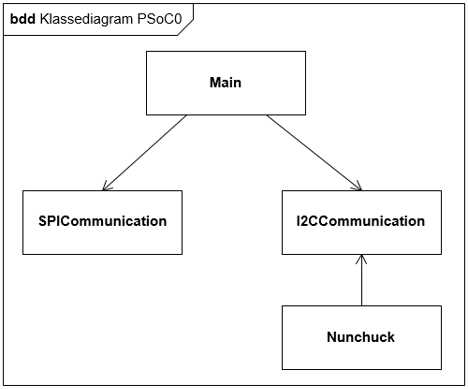
\includegraphics[width=.7\textwidth]{DesignOgImplementering/images/PSoC0KlassediagramOversigt}
	\caption{Klassediagram oversigt for PSoC0}
	\label{figure:klassediagramPSoC0}
\end{figure}

\begin{figure}[H]
	\centering
	\includegraphics[width=.7\textwidth]{DesignOgImplementering/images/PSoC1KlassediagramOversigt}
	\caption{Klassediagram oversigt for PSoC1}
	\label{figure:klassediagramPSoC1}
\end{figure}

\subsection{I2CCommunication}
I dette afsnit vil softwaren der omhandler I2C-kommunikation blive beskrevet. Dette inkluderer et klassediagram, samt en klassebeskrivelse.
\subsubsection{Klassediagram}
På figur \ref{figure:klassediagramI2CCommunication} ses klassediagrammet for I2CCommunication. 
\begin{figure}[H]
	\centering
	%\includegraphics[width=0.9\textwidth, trim={0 19cm 9cm 0},clip]{DesignOgImplementering/images/I2CCommunication.pdf}
	\includegraphics[]{DesignOgImplementering/images/I2CCommunication}
	%\includegraphics[width =0.9\textwidth]{DesignOgImplementering/images/I2CCommunication2}
	\caption{Klassediagram for I2CCommunication klassen}
	\label{figure:klassediagramI2CCommunication}
\end{figure}

\subsubsection{Klassebeskrivelser}
Som det ses på klassediagrammet figur \ref{figure:klassediagramI2CCommunication} indeholder klassen flere metoder. Disse metoder blive beskrevet her.\newline

\noindent\textbf{void sendData(uint8 Address, uint8 commandType, uint8* buffer, uint8 buffersize)}\newline
Denne metode sender, via PSoC Creators I2C-API, den data der ligger i "buffer" af kommandotypen "commandType" til slaven med adressen "Address". \newline

\noindent\textbf{void initReceiveData()} \newline 
Denne metode initialiserer de to buffers (slaveWrite og slaveRead) der kræves på en I2C-slave, for at kunne gøre bruge af PSoC Creator's I2C-API. \newline

\noindent\textbf{void receiveData(uint8* buffer)}\newline
Denne metode venter på at slaveRead bufferen er blevet fyldt. Når dette er sket, bliver slaveRead bufferen kopieret over i "buffer".   

\subsection{Nunchuck}
I dette afsnit vil softwaren der specifikt omhandler kommunikationen mellem PSoC0 og Nunchucken blive beskrevet. Dette gøres vha. et klassediagram og klassebeskrivelser.

\subsubsection{Klassediagram}
På figur \ref{figure:NunchuckKlassediagram} ses klassediagrammet for Nunchuck klassen.

\begin{figure}[H]
	\centering
	\includegraphics[]{DesignOgImplementering/images/nunchuck}
	\caption{Klassediagram for klassen Nunchuck}
	\label{figure:NunchuckKlassediagram}
\end{figure}

\subsubsection{Klassebeskrivelser}
Metoderne fra klassediagrammet figur \ref{figure:NunchuckKlassediagram} vil blive beskrevet i dette afsnit.

\noindent\textbf{int NunchuckSendHandshake()}\newline
Denne metode sender et "handshake" (Se dokumentationen afsnit \textbf{INSERT AFSNIT HER \#ref}) til Nunchuck enheden. Handshaket bruges til at "parre" PSoC'en med nunchucken. Metoden returnerer et '0' hvis der opstår en fejl. \newline

\noindent\textbf{int NunchuckRequestData()}\newline
Denne metode sender et 0x00 til nunchuck'en, og derved beder nunchuck'en om at klargøre data til overførsel. Metoden returnerer et '0' hvis der opstår en fejl. \newline

\noindent\textbf{int NunchuckreadData(uint8* buffer)}\newline
Denne metode bruger PSoC Creator's I2C-API til at læse data fra nunchuck'en (data der blev klargjort fra NunchuckRequestData()). Disse data bliver derefter dekrypteret og gemt i "buffer", så de bliver tilgængelige uden for metodens scope. \newline

I klassediagrammet er der en sektion kaldet "Defines". Disse Defines bruges i implementeringen til forskellige formål. \textit{PSoC0UnitAddress, PSoC1UnitAddres} og \textit{nunchuckUnitAddress} bruges til at definere adresserne for I2C-nettets slaver. \textit{NunchuckData, I2CTestRequest} og \textit{I2CTestACK} er kommando typer der bruges til at bestemme hvilken kommando type der er blevet sendt/modtaget, og hvor mange bytes der skal forventes at være gemt i databufferen (Se dokumentationen afsnit \textbf{INDSÆT REFERENCE TIL DOKUMENTATIONAFSNIT \#ref}) 

\subsection{SPI - PSoC}
I dette afsnit vil softwaren der specifikt omhandler SPI-kommunikationen mellem PSoC0 og DevKit8000 blive beskrevet. Dette gøres vha. et klassediagram og klassebeskrivelser

\subsubsection{Klassediagram}
På figur \ref{figure:KlassediagramSPICommunication} ses klassediagrammet over SPICommunication klassen.

\begin{figure}[H]
	\centering
	\includegraphics[]{DesignOgImplementering/images/SPICommunication}
	\caption{Klassediagram over klassen SPICommunication}
	\label{figure:KlassediagramSPICommunication}
\end{figure}
\subsubsection{Klassebeskrivelser}
I dette afsnit vil klassens metoder og defines blive beskrevet.
\newline

\noindent\textbf{void completeSPITest()} \newline
Denne metode gemmer \textit{SPI\_OK} i PSoC'ens SPI-transfer buffer. \newline

\noindent\textbf{void completeI2CTest()} \newline
Denne metode gennemfører I2C-Testen. Dette gøres ved at der sendes en besked til alle enheder på I2C-nettet, og hvis der ikke registreres nogen fejl på denne besked, bliver \textit{I2C\_OK} gemt i PSoC'ens SPI-transfer buffer. Registreres der en fejl, bliver \textit{I2C\_FAIL} gemt i SPI-transfer buffer. \newline

\noindent\textbf{void completeNunchuckTest(uint8* databuf)} \newline
Denne metode gennemfører Nunchuck-testen. Dette gøres ved at der startes en timer på 6 sekunder. Hvis der sker et tryk på 'Z'-knappen på nunchucken indenfor disse 6 sekunder, vil \textit{NUNCHUCK\_OK} blive gemt i SPI-transfer bufferen. Hvis der ikke registreres nogen tryk inden for de 6 sekunder, er det \textit{NUNCHUCK\_FAIL} der gemmes.\newline

I klassediagrammet er der beskrevet en række "Defines". Disse defines bruges i klassen som unikke ID'er der indikerer om en test er gennemført OK eller om den er fejlet.

\section{Afkodning af Wii-Nunchuck Data Bytes}
Aflæste bytes fra Wii-Nunchuck - indeholdende tilstanden af knapperne og det analoge stick - er kodet når de oprindeligt modtages via I2C bussen. Disse bytes skal altså afkodes før deres værdier er brugbare. Afkodningen af hver byte sker ved brug af følgende formel:

\textit{AfkodetByte = (AflæstByte XOR 0x17) + 0x17}

Fra formlen kan det ses at den aflæste byte skal \textit{XOR}'s (Exclusive Or) med værdien 0x17, hvorefter dette resultat skal adderes med værdien 0x17.

\section{Kalibrering af Wii-Nunchuck Analog Stick}
De afkodede bytes for Wii-Nunchuck's analoge stick har definerede standardværdier for dets forskellige fysiske positioner. Disse værdier findes i tabel \ref{tabel:WiiNunchuckStickPositioner}

\begin{table}[H]
	\centering
	\begin{tabular}{|l|l|}
		\hline
		X-akse helt til venstre & 0x1E \\ \hline
		X-akse helt til højre   & 0xE1 \\ \hline
		X-akse centreret        & 0x7E \\ \hline
		Y-akse centreret        & 0x7B \\ \hline
		Y-akse helt frem        & 0x1D \\ \hline
		Y-akse helt tilbage     & 0xDF \\ \hline
	\end{tabular}
	\caption{Standardværdier for fysiske positioner af Wii-Nunchuck's analoge stick}
	\label{tabel:WiiNunchuckStickPositioner}
\end{table}

I praksis skal de afkodede værdier for det analoge stick kalibreres, da slør pga. brug gør at de ideale værdier ikke rammes. 

I projektet er de afkodede værdier for det analoge stick kalibreret med værdien -15 (0x0F i hexadecimal), altså ser den endelige formel for afkodning samt kalibrering således ud:

\textit{AfkodetByte = (AflæstByte XOR 0x17) + 0x17 - 0x0F}

\section{Hardwaredesign}
På baggrund af BDD'et er der fundet følgende hardwareblokke, der skal udarbejdes: 
\begin{itemize}
	\item Motorstyring
	\item Tre motorer
	\item Affyringsmekanisme 
\end{itemize}
Disse beskrives i de følgende afsnit. 

\subsubsection{Motor}
Der er truffet et valg om at bruge en DC-motor i alle tre tilfælde. De to motorer skal bruges til at styre kanonen i to retninger, og den sidste skal bruges i affyringsmekanismen. 

\subsection{Motorstyring}
Til at styre de tre motorer er der bygget en H-bro, der skal bruges i tre eksemplarer. To af disse motorer skal kunne styre kanonen, så den ene gør at den kan køre op og ned, og den anden gør, at den kan køre fra side til side. Den tredje skal bruges til at styre affyringsmekanismen. 

\subsubsection{H-bro}
Der blev først designet en H-bro, som bestod af to N-MOSFET's af typen IRLZ44 og to P-MOSFET's af typen ZVP3306. Denne kan ses i bilaget. Det viste sig dog, at den P-MOSFET, der var brugt, var for svag til at kunne trække den strøm, som motoren skulle bruge, hvilket betød, at den blev brændt af. Derfor blev denne H-bro modificeret, så de to P-MOSFET's blev udskiftet med to MOSFET's af typen IRF9Z34N, der kan trække en større strøm. 

\begin{figure}[H]
	\centering
	\includegraphics[width=\textwidth]{DesignOgImplementering/images/motorkreds}
	\caption{Kredsløb for H-bro}
	\end{figure}

\begin{table}[]
	\centering
	\caption{Komponentbetegnelser på H-bro}
	\label{my-label}
	\begin{tabular}{|l|l|l}
		\cline{1-2}
		Betegnelse 	& Komponent 	          	 &  \\ \cline{1-2}
		VCC        	& 5V                         &  \\ \cline{1-2}
		Q1   		& IRLZ44(mosfet N-Channel)   &  \\ \cline{1-2}
		Q2   		& IRLZ44(mosfet N-Channel)   &  \\ \cline{1-2}
		Q3   		& IRLZ44(mosfet N-Channel)   &  \\ \cline{1-2}
		Q4   		& IRLZ44(mosfet N-Channel)   &  \\ \cline{1-2}
		Q5   		& BC547                      &  \\ \cline{1-2}
		Q6   		& BC557                      &  \\ \cline{1-2}
		Q7   		& BC547                      &  \\ \cline{1-2}
		Q8   		& BC557                      &  \\ \cline{1-2}
		Q9   		& IRF9Z34N(mosfet P-Channel) &  \\ \cline{1-2}
		Q10  		& IRF9Z34N(mosfet P-Channel) &  \\ \cline{1-2}
		R1   		& 10k$\Omega$                &  \\ \cline{1-2}
		R2   		& 10k$\Omega$                &  \\ \cline{1-2}
		R3   		& 10k$\Omega$                &  \\ \cline{1-2}
		R4   		& 10k$\Omega$                &  \\ \cline{1-2}
		R5   		& 10k$\Omega$                &  \\ \cline{1-2}
		R6   		& 100$\Omega$                &  \\ \cline{1-2}
		R7   		& 100$\Omega$                &  \\ \cline{1-2}
		R8   		& 10k$\Omega$                &  \\ \cline{1-2}
		D1   		& IN5819                     &  \\ \cline{1-2}
		D2   		& IN5819                     &  \\ \cline{1-2}
		D3   		& IN5819                     &  \\ \cline{1-2}
		D4   		& IN5819                     &  \\ \cline{1-2}
	\end{tabular}
\end{table}

\subsubsection{MOSFET'er}
Til at styre motoren er der bygget en H-bro, som består af fire mosfet, hvor to af dem er af typen IRF9Z34N (mosfet P-channel, som er Q9 og Q10 på kredsløbstegningen) og de to andre mosfet er af typen IRLZ44 (mosfet N-Channel, som er Q3 og Q4 kredsløbstegningen). Det er valgt at bruge mosfet for at kunne styre H-broen, da det ved denne er muligt at lukke og åbne for spændingen, og de bliver styret af spænding, i forhold til transistorer, som bliver styret af strøm. 

\begin{itemize}
\item MOSFET N-kanal\\
	Der er i denne H-bro brugt en N-kanals-MOSFET af typen IRLZ44. Denne MOSFET skal bruges til at trække strømmen fra den tilsvarende P-MOSFET til stel, så motoren kan begynde at køre. Det sker, når der kommer 5V ind på gate-benet. 
	\\MOSFET'en fungerer på den måde, at når der kommer positiv spænding ind på gate-benet åbner den, så der kommer forbindelse til stel og når der kommmer 0V ind på dette lukker den igen. 
	
	\begin{figure}[H]
		\centering
		\includegraphics[width=\textwidth]{DesignOgImplementering/images/grafn}
		\caption{Gate-to-Source Voltage REFERENCE TIL DATABLAD HER!!!!}
	\end{figure}
	
	På figur (reference her!) ses det, at når der er en gate-to-source-spænding på 5V, vil der MOSFET'en kunne klare, at der løber en strøm på op til 100A/30A (TJEK DETTE!!). Det vil altså ikke komme til at påvirke motoren, da denne kun kan trække en strøm på cirka 0,35A. 
	
\item MOSFET P-kanal \\
	Der er valgt at bruge en P-MOSFET af typen IRF9Z34N. Denne MOSFET skal bruges til at trække de 12V ned til motoren, så denne kan køre. Samtidig sørger den for, at de 12V ikke løber ned til motoren så længe, der ikke er negativ spænding på gate-benet. 
	Denne type MOSFET kan trække en strøm på 6,7A ifølge databladet. Det vil altså ikke komme til at påvirke motoren, da den kun kan trække en strøm på cirka 0,35A. 
	
	For at der kan løbe spænding igennem IRF9Z34N, skal den have en negativ spænding for at åbne og en spænding på over 0V for at lukke. 
		
	\begin{figure}[H]
		\centering
		\includegraphics[width=\textwidth]{DesignOgImplementering/images/grafp}
		\caption{Gate-to-Source Voltage REFERENCE TIL DATABLAD HER!!!!}
	\end{figure}
	
	På figuren (REFERENCE HER!) ses det, at når der er en gate-to-source-spænding på 5V, vil derr kunne løbe en strøm på omkring 5A igennem MOSFET'en, hvilket er mere end nok til at få motoren til at køre. 
	
\end{itemize}

\subsubsection{Dioder}
Over fire af mosfetene (Q9, Q10, Q3 og Q4) er der sat en diode af typen IN5819. Den skal fungere som beskyttelse af de fire mosfet (Q9, Q10, Q3 og Q4). Det, de gør, er, at de sikrer, at den spænding, som er tilbage i motoren, når man lukker for mosfetene, ikke løber tilbage ind i mosfetene og brænder dem af.

\subsubsection{Modstande}
\begin{itemize}
	\item Pull down modstande:\\
	Der er blevet brugt fire pull-down-modstande (R1, R2, R3 og R4). Disse sørger for, at signalet vil blive holdt lavt, når der ikke er trykket, så dette ben ikke står og flyver, så det kan komme til at åbne en mosfet ved en fejl og derved kommer til at brænde en mosfet eller motoren af. Der er valgt en modstand på 10 kOhm, hvilket betyder, at den er lille nok til at trække de små spændinger ned, når der ikke er trykket, og den stor nok til at spændingen ikke løber derned, når der er trykket. 
	\item Andre modstande
	\begin{itemize}
		\item R6 og R7\\
			Grunden til, at R6 og R7 er der, er for at sikre, at transistorernes Absolute Maximum Ratings omkring strømmen, som ikke må overstige 100mA ifølge databladet. (tjek lige om det er rigtig)
		\item R5 og R8\\
			Grunden til at R5 og R8 er sat ind i kredsløbet er, at der ifølge databladet kun kan løbe en strøm på omkring 30A igennem den N-MOSFET, der er brugt, Vgs er 10V. Da Vgs kun er sat til 5V, vil MOSFET'en altså ikke kunne klare en alt for stor strøm. Derfor er R5 og R8 sat ind for at forhindre, at MOSFET'en ikke brænder af. 
	\end{itemize}

\end{itemize}

\subsubsection{Transistorer}
\begin{itemize}
	\item Q5 og Q7
	Disse transistorer sidder i kredsløbet, fordi det tager tid for P-MOSFET'en at blive opladt helt, på grund af kondensator effekt imellem benene på mosfet'en, for ellers ville den tag for lang tid om at åbne helt. Det hjælper den disse transistorer til med. 
	
	\item Q6 og Q8
	Disse to transistorer sidder der for at hjælpe med at lukke P-MOSFET'en igen. Inden Q5 og Q7 blev sat ind tog det tid for at lukke P-MOSFET'en, men da de to blev sat ind, kunne de hjælpe til med at aflade mosfet'ene hurtigere. Derfor sidder de der, for at IRF9Z34N kan lukke hurtigt. 
\end{itemize}
\subsubsection{Potentiometer}
For at kunne holde styre på at motoren ikke bare drejer hele vejen rundt, men holder sig inde for de grænser som blev fast sat i kravspecifikationen, er der blevet valgt at bruge et potentiometer, som virker på den måde at man kan ændre på modstandsværdien i selv potentiometeret, så man kan få en laver spænding ud, der ved kan man styre hvor langt motoren er drejet over til den ene side ved kun at kigge på selv spændingen fra potentiometeret. For at regne ud hvor langt motoren er, kan man regne ud hvor meget spænding der kommer ud ved at bruge spændingsdeler formlen, som er vist på figur \ref{fig:potentiometer2}
\begin{figure}[H]
	\centering
	\includegraphics[width=\textwidth]{DesignOgImplementering/images/potentiometer}
	\caption{spændigsdeler formlen hvordan den virker i potentiometere}
	\label{fig:potentiometer2}
	
\end{figure}
Hvor man se Rtop og Rbottom, som en modstand, men den bliver delt af midter strengen, som fortæller hvor modstanden skal deles henne og som man kan se på formlen ved side af, kan man se hvor meget spænding som kommer ud af den. 
Det potentiometer som bliver brugt i dette projekt er 47Kohm, som er linæret vil spændingen stiger lige meget hver gang man drejer på potentiometeret

\begin{figure}[H]
	\centering
	\includegraphics[width=\textwidth]{DesignOgImplementering/images/udpot}
	\caption{udregning for potentiometer}
	\label{fig:pot}
	
\end{figure}
Så dvs når potentiometeret står i midten vil der komme en spænding ud på ca 2.5V, så når spændingen bliver lavere vil der komme et punkt hvor motoren ikke vil kunne køre til den ene side mere og det samme sker når man hæver, vil motoren ikke kunne køre den anden vej. 
Der er blevet målt med en vinkel måler for at over holde kravene i 

\subsubsection{ADC}
For at kunne læse hvad spænding er på potentiometeret, så bliver der brugt i dette projekt ADC af typen Sequencing Successive Approximation ADC. Som funger på denne måde at 
det er et sample hold kreds, som vil sige at den holder på et signal end til den er klar på at tag et nyt signal ind. Så den har tid til at finde frem til hvilken værdi, som den skal konverter til, er ved at sættet DAC til midscale og tjekke om inputtet er højre eller lavere end hvor midscaler er. Hvis den er højere får den 1 og hvis den er laver for den et 0, det bit bliver gemt i et register. Så finder man nu midten i mellem midscale og den øvre halvdel eller nedre halvdel af skalaen og sådan bliver man ved end til alle bit er blevet sat. Så tjekker man registeret for at læse hvilket tal som er fundet, ved at læse fra MSB(most significant bit) til LSB(least significant bit) og det er tal som man har sat på indgangen. På figuren\ref{fig:ADC1} kan man få et bedre overblik over hvordan ADC funger. 

\begin{figure}[H]
	\centering
	\includegraphics[width=\textwidth]{DesignOgImplementering/images/ADC}
	\caption{Hvordan ADC virker}
	\label{fig:ADC1}
	
\end{figure}

Jo flere bit man har jo mere præcise bliver det også, men man kan godt risiker at man er 1LSB over/under det resultat man skal have, men for dette projekt gør det ikke noget om man 1 LSB over/under.

	\chapter{Test}
For at verificere systemets funktionaliteter for både hardware og software blev der udført modultests, integrationstests samt en endelig accepttest af de to use cases. Følgende tabel giver en oversigt over hvilke tests, der er blevet udført, samt en reference til hvor i dokumentationen testbeskrivelsen findes.

\begin{table}[H]
	\centering
	\label{test}
	\begin{tabular}{|l|l|l|}
		\hline
		\textbf{Test}      & \textbf{Reference} & \textbf{Side}\\ \hline
		Wii-Nunchuck        & 5.1.1 & 94              \\ \hline
		SPI Protokol        & 5.1.2 & 96              \\ \hline
		I2C Protokol        & 5.1.3 & 97             \\ \hline
		Systemtest GUI   & 5.1.4 & 100               \\ \hline
		Rotationsdetektor   & 5.1.5 & 102             \\ \hline
		H-bro               & 5.2.1 & 104             \\ \hline
		Rotationsbegrænsing & 5.2.2 & 107              \\ \hline
		Rotationsdetektor   & 5.2.3 & 110             \\ \hline
		Integrationstest    & 5.3 & 120                \\ \hline
		Accepttest          & 6 & 124                  \\ \hline
		
	\end{tabular}
	\caption{Referencer til test afsnit}
\end{table}

\noindent \textbf{Modultest} \newline
\noindent Ved modultests blev én funktionalitet testet isoleret. Det vil sige med så lidt påvirkning fra resten af systemet som muligt. Modultests blev udført før integrationstests, for at sikre individuel funktionalitet før sammensætning af alle komponenter. Modultests blev udført både for software- og hardwarekomponenter. \newline

\noindent \textbf{Integrationstest} \newline
\noindent Ved integrationstesten blev alle elementer, der er inkluderet i use case 2, sammensat og systemet som helhed blev testet. Værdien af dette var, at alle hardware- og softwaremoduler som førhen kun var testet i isolation, blev testet i sammenhæng med andre moduler.  \newline

\noindent \textbf{Accepttest} \newline
\noindent I samarbejde med vejlederen er der foretaget en accepttest af prototypen. Værdien af dette var, at test om alle de krav, der blev stillet til produktet, var overholdt.

	%\chapter{Udviklingsværktøjer}

\section{PSoC}

\section{DevKit 8000}

\section{QT Creator}
QT Creator er blevet brugt til at designe brugergrænsefladen.
QT's design widget suite/API er blevet brugt som den primære del af QT frameworket. Det fungerede godt til at designe en EDP-baseret grænseflade. Frameworket's indbyggede beskedsystem passede godt til vores design.
En knap er assignet til et slot i brugergrænseflade-klassen, og når der trykkes på den pågældende knap, bliver det assignede signal broadcastet, og slot-funktionen bliver kørt.
Design suiten simplificerer selve programmeringen af grænsefladen. Det skjuler mange af funktioner under kølerhjelmen.

Liste:
PSoC Creator
Analog discovery

	%\chapter{Resultater og Diskussion}

\chapter{Resultater}
\label{afsnit:resultater}

I slutningen af produktudviklingen blev der afviklet en accepttest i samarbejde med gruppens vejleder Gunvor Elisabeth Kirkelund. Denne udfyldte accepttest kan ses i dokumentationen, afsnit 6-\textit{Udfyldt Accepttest} side 124.

\noindent På tabel \ref{table:UseCaseResults} ses en opsummering af resultaterne fra produktets udførte accepttests. 

\begin{table}[H]
	\centering
\begin{tabular}{|l|l|}
	\hline
	Use Cases                                   & Resultat                                                                           \\ \hline
	Use Case 1 - Spil Goofy Candygun 3000       & \begin{tabular}[c]{@{}l@{}}Denne use case er\\ delvist implementeret.\end{tabular} \\ \hline
	Use Case 2 - Test kommunikationsprotokoller & \begin{tabular}[c]{@{}l@{}}Denne use case er\\ implementeret.\end{tabular}         \\ \hline
\end{tabular}
	\caption{Opnåede resultater for systemets use cases}
	\label{table:UseCaseResults}
\end{table}

\noindent Use case 1 er delvist implementeret, da brugergrænsefladen er implementeret som en demo. Der er ingen bagomliggende funktionalitet til at vise spillets statistikker, samt administrering af player-modes. Der er en slik kanon som kan styres med en Nunchuck, og affyringsmekanismen kan aktiveres. Dog mangles kalibrering af motor og affyringsmekanisme, da motoren ikke kan bære kanonens vægt, og slik ikke kan affyres med tilstrækkelig kraft. \newline

\noindent Projektforløbet resulterede i en prototype hvor use case 1 og use case 2 er implementeret som beskrevet.


	\chapter{Fremtidigt arbejde}

Et problem ved produktet er, at affyringsmekanismen er meget tung i begge ender, så hvis der drejes for langt ud med Wii-nunchuck vipper den enten frem eller tilbage. Dette ville kunne have været afhjulpet med en H-bro. Denne ville nemlig så kunne have bremset affyringsmekanismen ved at være blevet sat til at køre i begge retninger i den tid, den skal holde stille. Hvis denne H-bro skulle medtages i systemet skulle der også skrives noget software, hvor H-broen blev sat til at køre i begge retninger på samme tid. 

Noget andet der kan arbejdes videre med, er noget i samme stil som med bremsefunktionen af affyringsmekanismen. Problemet er, at affyringsmekanismens motor ikke kører særligt stærkt. Det skyldes, at rotationsdetektoren ikke kunne nå at stoppe motoren, inden den havde kørt en omgang mere. For at afhjælpe det problem blev motorens dutycycle sat ned, men det gjorde, at affyringsmekanismen nu ikke længere kunne skyde særligt hårdt. Derfor ville det være en god ide, at bruge en H-bro til også at styre denne motor, så den kunne få en bremsefunktion, ligesom den vertikale drejefunktions. 
	%\include{Afsnit/FejlOgMangler/FejlOgMangler}
	\chapter{Konklusion}
Der blev i dette projekt brugt scrum som en udviklingsmodel, da denne model kan håndtere ændringer i krav til produktet eller design under projektforløbet. Derved var det muligt at arbejde iterativt, da man kunne tage hensyn for nye ændringer i et nyt sprint. \newline

 \noindent For hver sprintopstart blev der bestemt opgaver til udførelse samt tidsestimering af disse. Sprintvarigheden var på 3 uger, hvilket gjorde, at man fik et delmål for projektet der skulles udvikles på i sprintet. Det gav en følelse af fremskridt efterhånden som projektet skred fremad. Ved at arbejde i sprint blev projektet delt op i små dele. Dette var en fordel da de små delmål var lettere at starte med end at starte med et stort mål. \newline 
 
 \noindent En del af scrum var daglige stå op møder. I løbet af projektet skiftede gruppen mellem forskelle måder at afholde disse møder. Efter forskellige forsøg fandt vi ud af, at det fungerede bedst når disse møder blev afholdt gennem en gruppesamtale på Facebook. Disse input gav alle et overblik over, hvad vi hver især arbejdede med på dagen, og det der var foretaget dagen forinden. \newline
  
 \noindent I løbet af projektet har rollen som scrummaster skiftet for hvert sprint. Dette har fungeret gnidningsfrit og alle der ville prøve rollen, havde chancen for dette. \newline
 
 \noindent Under dette projektforløb har gruppen fået indsigt i den praktiske anvendelse af scrum og hvordan dette kan anvendes i forbindelse med fremtidige semesterprojekter. 

 



 




	\chapter{Referencer}

\begin{thebibliography}{9}
	
	\bibitem{I2C}
	UM10204,
	\textit{I2C Bus Specification and user manual}, 4 April 2014
	
	\bibitem{nunchuck}
	CSE325\_Assignment\_6\_F10,
	\textit{I2C Interface with Wii Nunchuck}, CSE325 Embedded Microprocessor Systems
	
	
	\bibitem{cmosStandard}
	Logic Signal Voltage Levels,
	\textit{All about circuits},
	Kuphaldt Tony R.,\newline
	\url{http://www.allaboutcircuits.com/textbook/digital/chpt-3/logic-signal-voltage-levels/} 
	Besøgt 22 Marts 2016
	
	
\end{thebibliography}
\end{document}	